\section{Simulation results}

\begin{figure}[H]
    \centering
    \includegraphics[width=1\textwidth]
    {fig/simplotssamlet.pdf}
    \caption{Simulation experiment results.}
\end{figure}

\section{Experimental results}

\subsection{Broadband light source}

The measurements on our silicon structures resulted in some difficulties. \\

The first measurements were performed with a broadband light source which produces two different LEDs simultaneously with their peak wavelengths at 1430 nm and 1550 nm respectively. The data for our 6 structures all had an ongoing problem as seen in Figure \ref{fig:Lightsource1Rep}. \\ 

\begin{figure}[H]
    \centering
    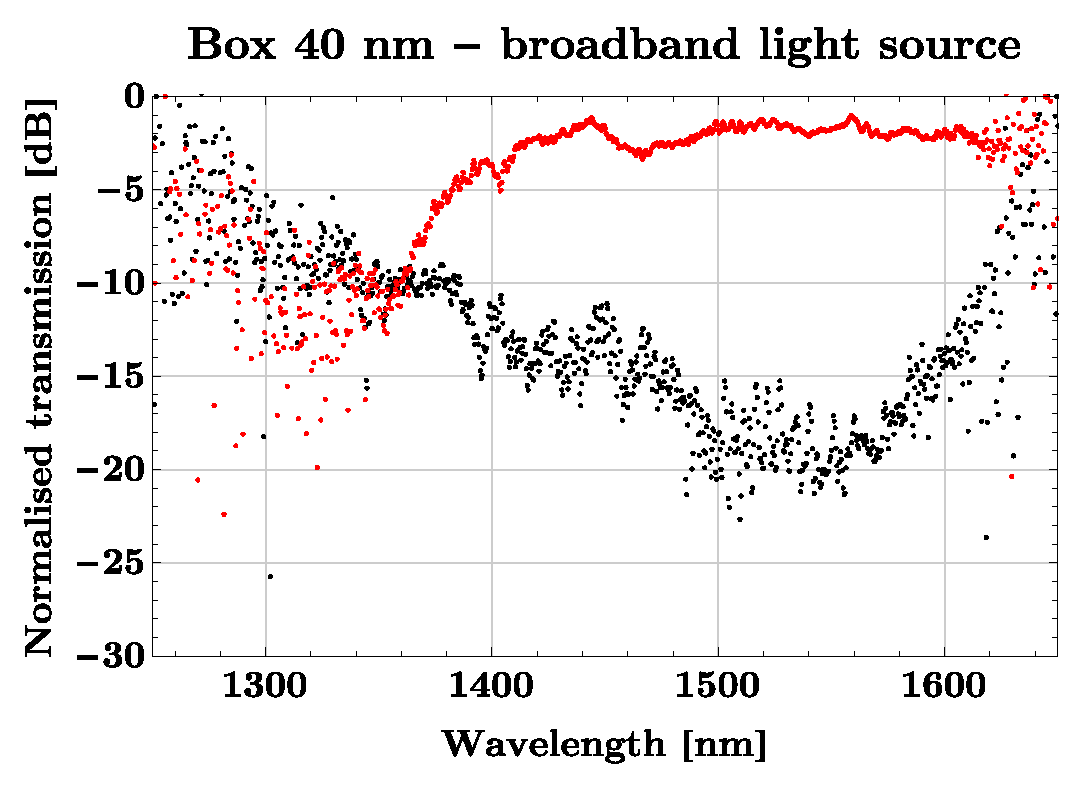
\includegraphics[width=0.8\textwidth]
        {fig/Kilde1Broadband/box40broadband.pdf}
    \caption{Data from box structure w. minimum feature size of 40 nm from a broadband light source.}
    \label{fig:Lightsource1Rep}
\end{figure}

As shown in the right side of FIG \ref{fig:Lightsource1Rep}, we have a significantly stronger signal around 1550 nm in our lower output waveguide, which matches our intuition, since the light source has the higher peak  at this wavelength and our structure is designed to filter light into 1300 nm and 1550 nm. Although in the left side of FIG \ref{fig:Lightsource1Rep} it is difficult to conclude anything from the data. It is assumed that the default in the data for lower wavelengths is caused our light source. The 1300 nm wavelength is too far from the 1430 peak wavelength that the LED produces, which means that the data is primarily affected by background noise. \\

\subsection{Multimeter light source}
Next we tried to change the light source to a multimeter which individually produces light with peak wavelength at 1310 nm and 1550 nm respectively which yielded a different but just as problematic problem as seen on FIG \ref{fig:Lightsource2Rep}. 

\begin{figure}[H]
    \centering
    \includegraphics[width=0.8\textwidth]
    {fig/Kilde2Multimeter/box40multimeter.pdf}
    \caption{Data from box structure w. minimum feature size of 40 nm from a multimeter.}
    \label{fig:Lightsource2Rep}
\end{figure}

Here we see a good signal on both sides for the light we designed the structure to let through, but since the two individual LED light sources in the multimeter does not send the full range of light, we cannot conclude that the structure filters unwanted light out because of the dominating background noise. This means, that even though we have a good transmission for 'wanted' wavelengths, we do not how well the crosstalk has been minimised.

\subsection{Multimeter light source, concatenated results}

To investigate the crosstalk, we performed measurements where we sent the 'unwanted' signal through the device, e.g. we sent light with a peak wavelength of 1550 nm through the device, and measured the output signal at the channel that favors light with wavelength at 1300 nm.

We then concatenated the useful regions of the results, i.e. in FIG \ref{fig:Lightsource2Rep} the data points from 1200 nm to 1400 nm were measured with the light source peaking at 1310 nm, the data points from 1400 nm to 1650 nm were measured with the light source with peaking at 1550 nm.

This method led to more useful results. We can now see in FIG \ref{fig:Kasse40nmKilde2Concatenated} that the box structure w. minimum feature size of 40 nm is working as intended. The high wavelengths are handled well: in the interval 1400 nm - 1650 nm, the signal is lowered by 4 dB at worst. Low wavelengths cause some trouble; the maximum output in the upper channel is lowered by 4 dB. 
\begin{figure}[H]
    \centering
    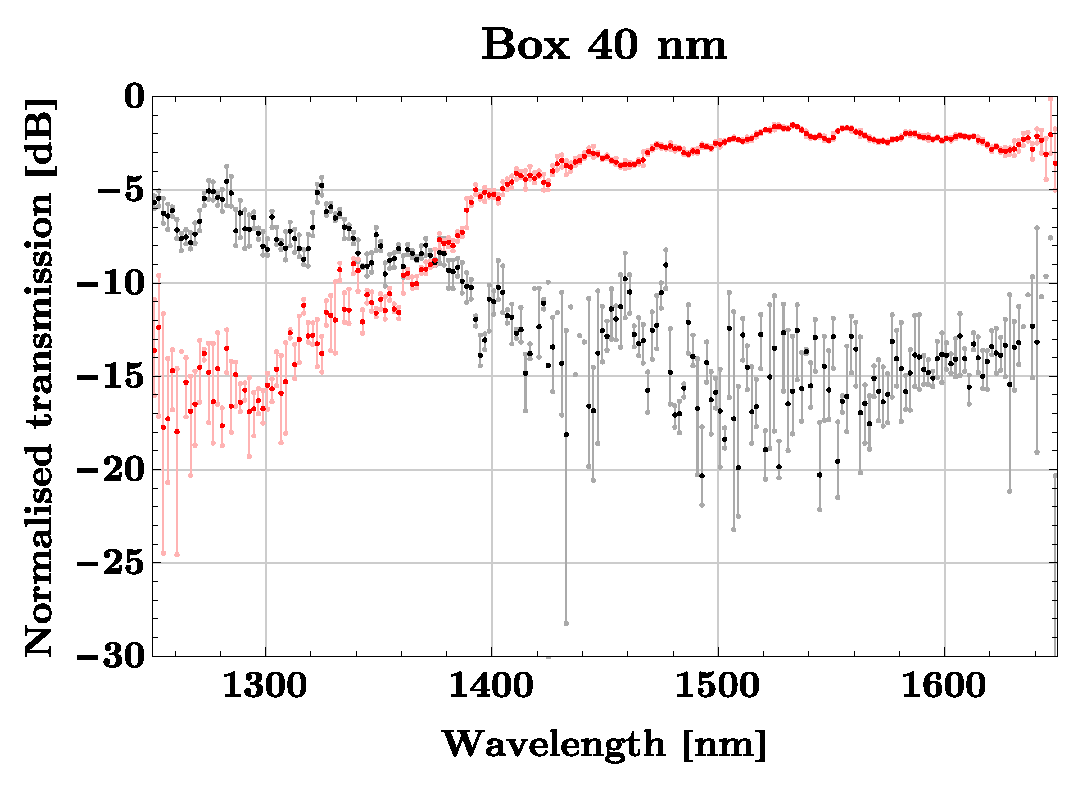
\includegraphics[width=0.8\textwidth]
    {fig/Kilde2Multimeter/box40multimeterconcatenated.pdf}
    \caption{Concatenated data from box structure w.  minimum feature size of 40 nm from a multimeter.}
    \label{fig:Kasse40nmKilde2Concatenated}
\end{figure}

The box structure w. minimum feature size of 60 nm performs more consistently (FIG \ref{fig:Kasse60nmKilde2Concatenated}): Maximum signals in the designated channels are lowered by roughly 5 dB, while the unwanted signals are lowered roughly 10 dB or better.

\begin{figure}[H]
    \centering
    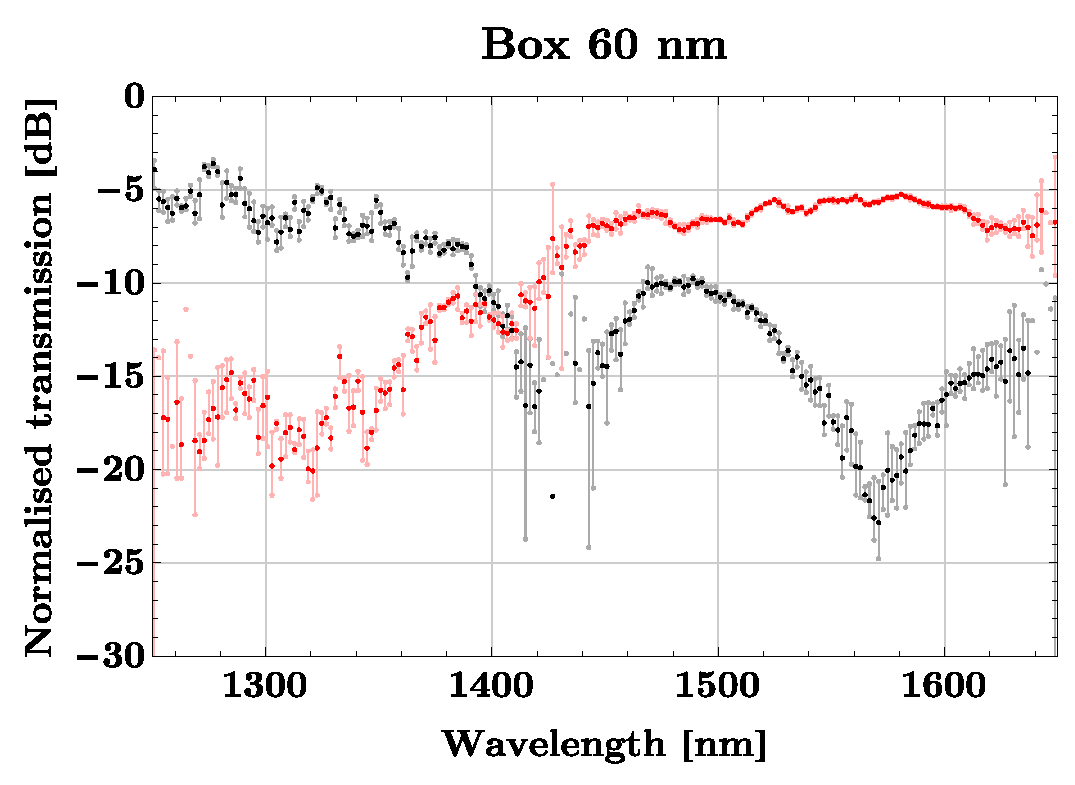
\includegraphics[width=0.8\textwidth]
    {fig/Kilde2Multimeter/box60multimeterconcatenated.pdf}
    \caption{Concatenated data from box structure w.  minimum feature size of 60 nm from a multimeter.}
    \label{fig:Kasse60nmKilde2Concatenated}
\end{figure}

The best-performing Y-junction structure (feature size 40 nm) does not outperform the box-structure. Apparently manually altering the initial structure to a Y-junction did not improve the performance of the device.

\begin{figure}[H]
    \centering
    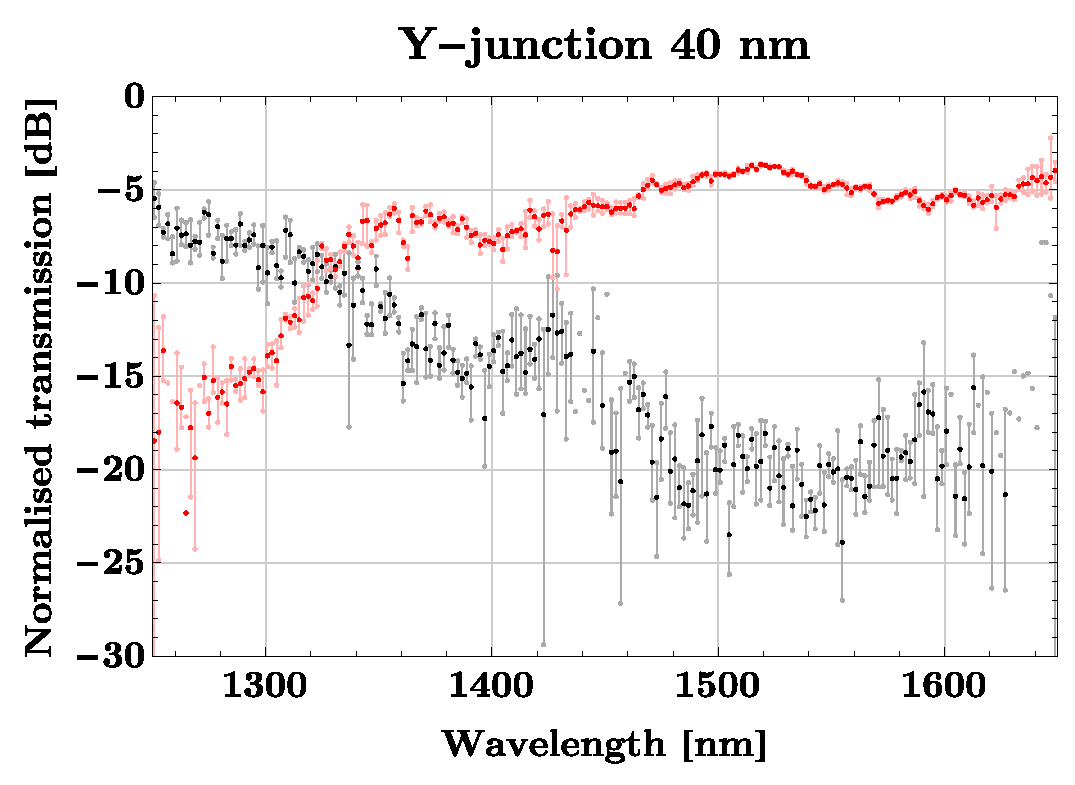
\includegraphics[width=0.8\textwidth]
    {fig/Kilde2Multimeter/yjunc40multimeterconcatenated.pdf}
    \caption{Concatenated data from Y-junction structure w. minimum feature size of 40 nm from a multimeter.}
    \label{fig:Yjunc40nmKilde2Concatenated}
\end{figure}